\section{Snowball System}

The \emph{Snowball} system\cite{Agichtein.Gravano:2000}(Figure \ref{fig:snowball}) provides a novel framework to generate patterns and extract tuples from documents iteratively. Also, it proposes strategies for evaluating the quality of extracted patterns and tuples. Only those "sufficiently reliable" patterns are qualified to extract candidate new tuples, and only those "sufficiently confident" tuples are kept by \emph{Snowball} as seed tuples for further iteration of the system. This bootstrapping framework for both extracting and filtering tuples significantly improve the quality and coverage of extracted results.

However, The \emph{Snowball} system can hardly be applied to PPI extraction task directly for three reasons:\\

(1)First, there is an assumption in \emph{Snowball} system that each tuple is unitary, taking organization-location tuple $\langle ORGANIZATION,LOCATION\rangle$ for an example, which means the headquarter of an \emph{organization} in located on certain \emph{location}. if \emph{organization} is known, say "Microsoft", then it becomes a undeniable fact that the \emph{location} would be bound to "Redmond". While in scenario of PPI information, it is by no means the same case. For example, given an incomplete tuple $\langle p53,?\rangle$, there is no certain answer. Perhaps it stands for the binding interaction within $\langle p53,p21\rangle$, or perhaps it presents the inactivation association within $\langle p53,XAF1\rangle$, or perhaps it indicates the up=regulation within $\langle p53,ML-1\rangle$. No certain answer pale the effectiveness and accuracy when evaluating the extracted results. Hence, a more sophisticated evaluation strategy is required.\\

(2)Second, given a set of seed tuples, no matter how large the set is, only a small fraction of patterns can be extracted, let alone the number of patterns which are regarded to be "sufficiently reliable", the qualified patterns is much scarcer. On one hand, the deficiency of pattern might bring about the \emph{Snowball} system to converge too soon, with scanty satisfactory new PPI extracted and significant low recall. On the other hand, if we compromise to decrease the evaluation criterion, though pattern number would flourish, the precision would be jeopardized. How to find more patterns without suffering from extraction quality downfall becomes a challenge.\\

(3)Third, \emph{Snowball} system requires to traverse all documents to find candidate patterns and tuples at each iteration. It would be rather time-consuming and computational-intensive to do so. Considering total literatures available in PUBMED exceed 30 million, so it is essential to figure out an optimization strategy for extraction efficiently.\\

\begin{figure}
\centering
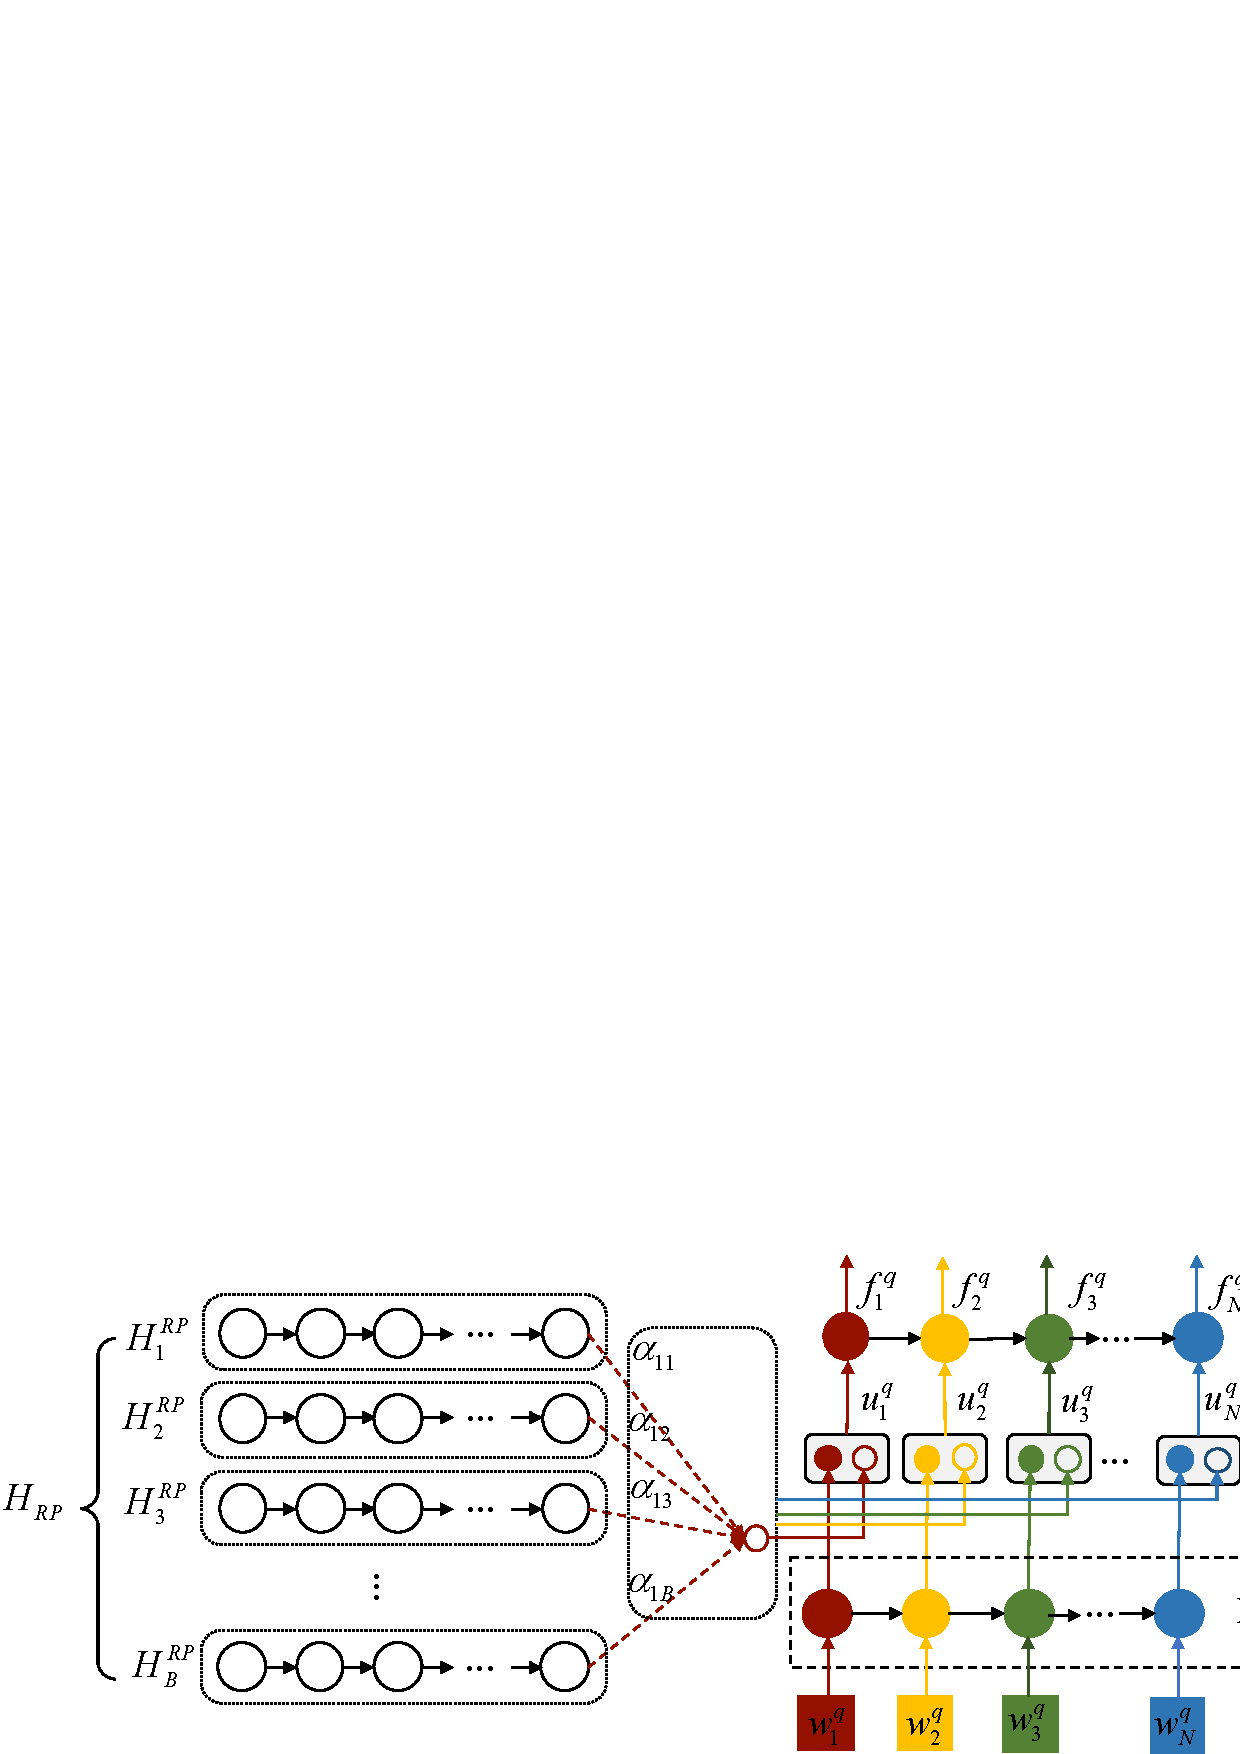
\includegraphics[totalheight=1.4in]{fig/figure1.png}
\caption{The main components of Original Snowball}
\label{fig:snowball}
\end{figure}

\begin{figure}
\centering
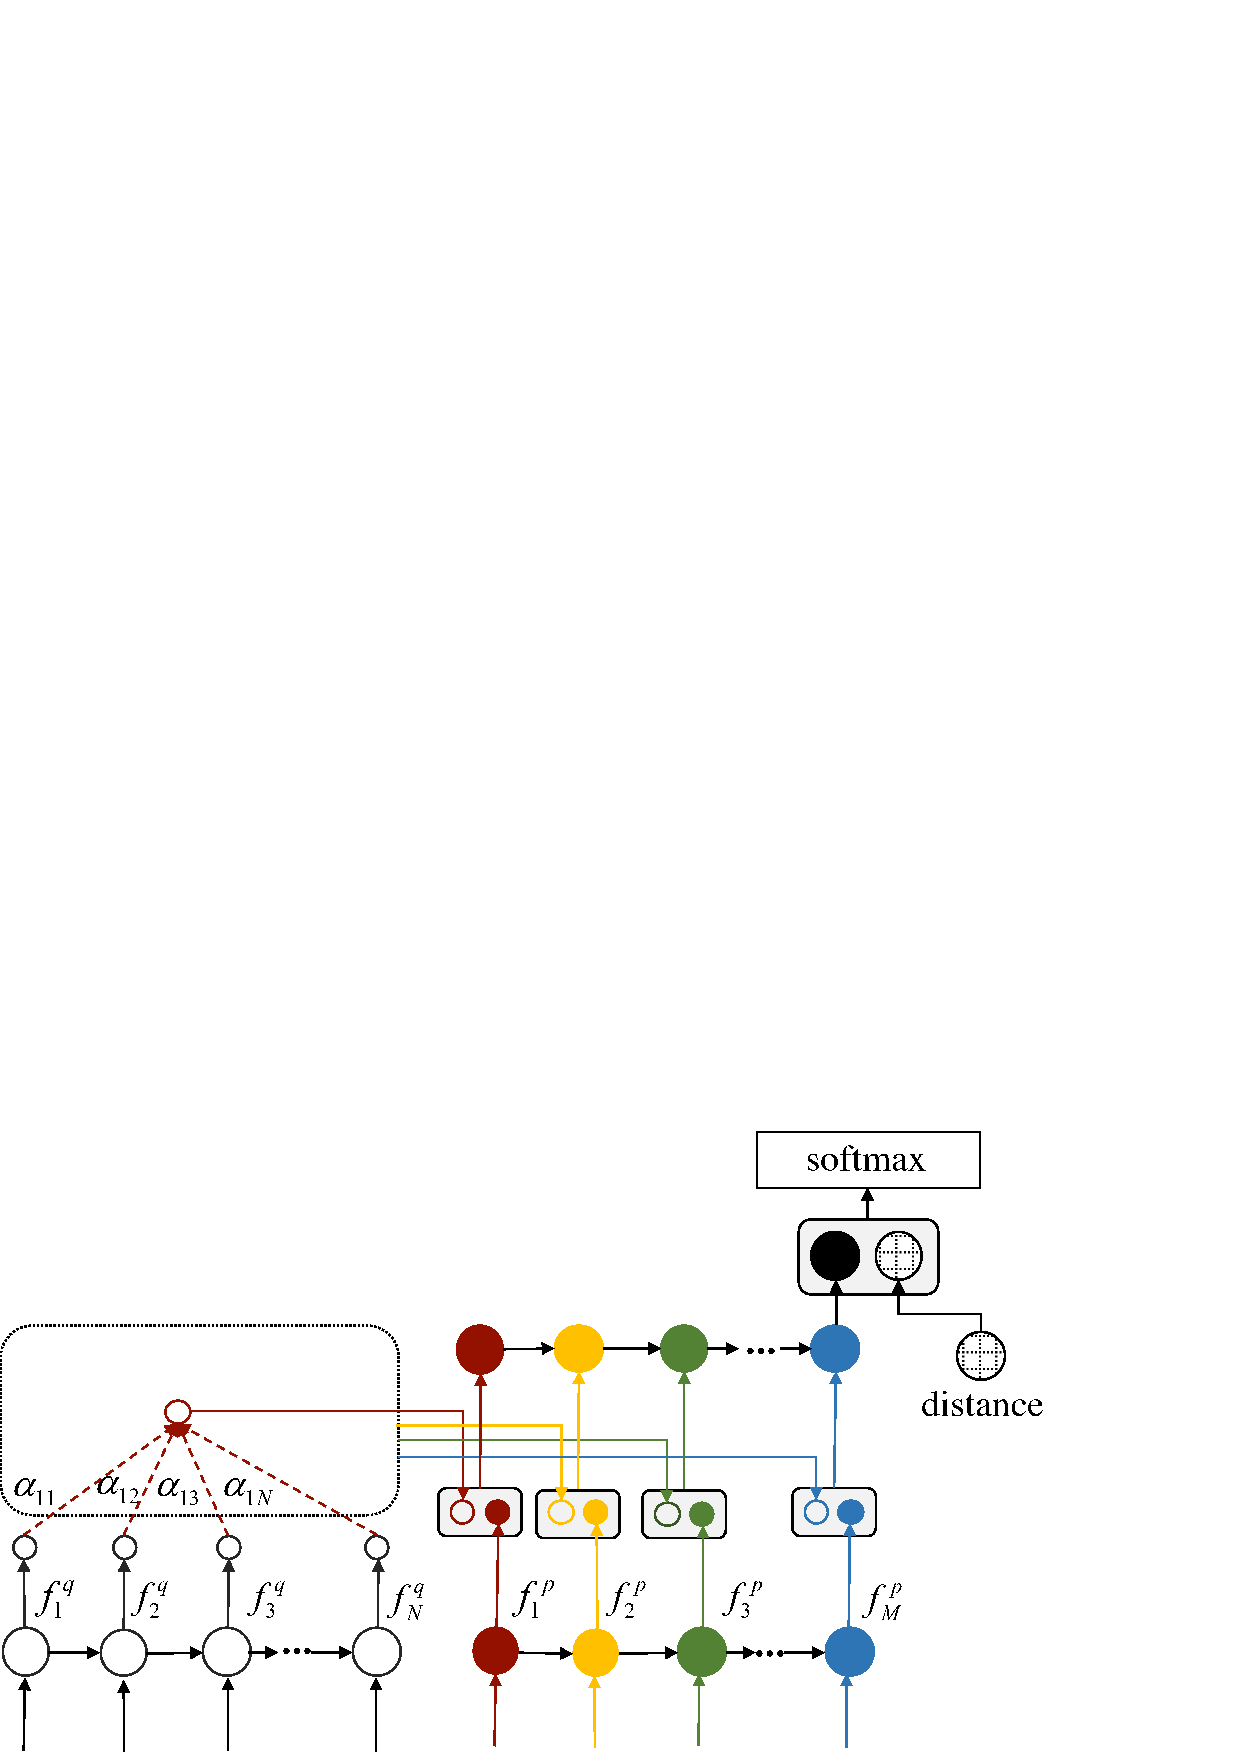
\includegraphics[totalheight=1.6in]{fig/figure2.png}
\caption{Workflow of PPISnowball}
\label{fig:ppisnowball}
\end{figure}
